% ----------------------------------------
% Chap: Versuche auf dem EHD-Messgerät
% ----------------------------------------
\chapter{Versuche auf dem EHD-Messgerät}
\label{chap:versuche_auf_dem_ehd_messgeraet}

% ----------------------------------------
% Sec: Versuchte Öle
% ----------------------------------------
\section{Versuchte Öle}
\label{sec:versuchte_oele}

Um die Funktionsfähigkeit des neuen Messsystem zu überprüfen, wird es mit verschiedenen Schmierstoffe getestet.

\paragraph{Schmierstoff 1}
\label{par:schmierstoff_1}

\begin{itemize}
    \item Firma
    \item Grund für das Öl
    \item Anwendungsbereiche
    \item technische Daten, kinematische Viskosität bei 40 und 100 Grad Celsius
\end{itemize}

\paragraph{Schmierstoff 2}
\label{par:schmierstoff_2}

\begin{itemize}
    \item Firma
    \item Grund für das Öl
    \item Anwendungsbereiche
    \item technische Daten, kinematische Viskosität bei 40 und 100 Grad Celsius
\end{itemize}

% ----------------------------------------
% Sec: Kapazitive Messgeräte zur Schmierfilmdickenbestimmung
% ----------------------------------------
\section{Kapazitive Messgeräte zur Schmierfilmdickenbestimmung}
\label{sec:kapazitive_messgeraete_zur_schmierfilmdickenbestimmung}

% ----------------------------------------
% Sub: Stromladekurve Messgerät
% ----------------------------------------
\subsection{Stromladekurve Messgerät}
\label{sub:stromladekurve_messgeraet}

Im IMKT gibt es ein mobiles Messsystem zur Schmierfilmdickenmessung mittels kapazitiven Messverfahren.
Das System besteht aus einem Laptop, der mit \textit{Laderkurve-Software} installiert, und einer Messkarte (Typ USB-6211) von der Firma National Instrument (NI).

Bei kapazitiver Messmethode wird der EHD-Kontakt als ein Kondensator ($C_K$) betrachtet.
Die Auflade des Kondensators erfolgt durch eine Ladespannung $U_L$ (\SIrange{0,2}{0,5}{\volt}) und einen Vorwiderstand $R_V$ (\SI{1015}{\kilo\ohm}).
Eine unendliche Erhöhung der Ladespannung ist aber unerwünscht, weil die zur Ionisierung des Schmierstoffes bei hohen Spannung verursacht und das kann die Messergebnisse verfälschen.
Abbildung \ref{fig:Schematischer_aufbau_des_mobilen_messsystems} zeigt das Prinzip des mobilen Messsystems zur Schmierfilmdickenmessung bei IMKT an.
% ----------------------------------------
% Fig: Schematischer Aufbau des mobilen Messsystems
% ----------------------------------------
\begin{figure}[htb]
    \centering
    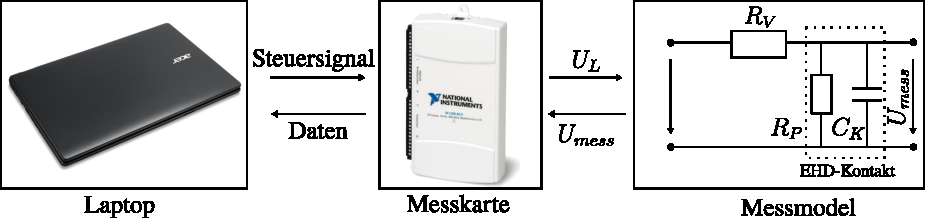
\includegraphics[]{./images/schematischer_aufbau_des_mobilen_messsystem.pdf}
    \caption{Schematischer Aufbau des mobilen Messsystems}
    \label{fig:Schematischer_aufbau_des_mobilen_messsystems}
\end{figure}

Das ganze Messsystem wird von der \textit{Laderkurve-Software} gesteuert.
Sie miss nicht direkt die Kapazität, sondern nimmt sie die Antwort bzw. Ladekurve des ``Kondensators'' auf, danach wird die Auswertung mit einem Matlab-Skript ausgeführt.
Die Software kann die Ladekurve in zwei Modi: \emph{Anzahl der Messwerte} oder \emph{Messung nach Zeit} aufnehmen.
Im Rahmen dieser Arbeit werden alle Messungen mit dem ersten Modus gemacht.
Abbildung \ref{fig:gui_der_laderkurve_software} zeigt die Benutzeroberfläche der Ladekurve-Software bei einer Testmessung mit einem Referenz-Kondensator (\SI{3.3}{\nano\farad}) an.
% ----------------------------------------
% Fig: GUI der Ladekurve-Software
% ----------------------------------------
\begin{figure}[htb]
    \centering
    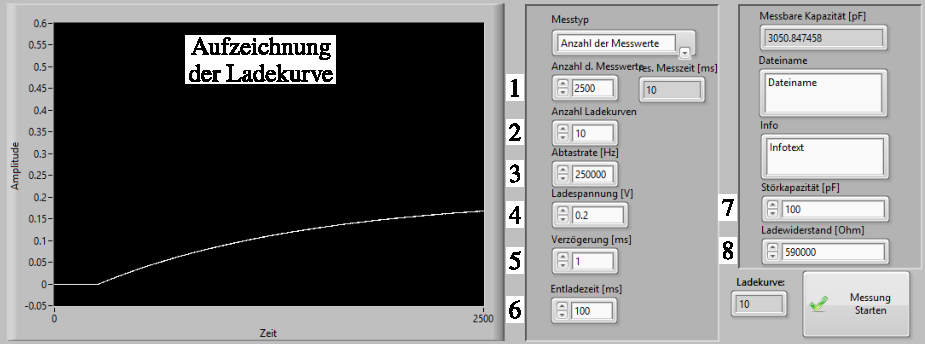
\includegraphics[]{./images/ladekurven_gui.pdf}
    \caption{Benutzeroberfläche der Laderkurve-Software}
    \label{fig:gui_der_laderkurve_software}
\end{figure}

Die Software ist relative einfach zu bedienen, allerdings gibt es folgende Punkte, auf die man beachten muss.
\begin{description}
    \item[1. Anzahl der Messwerte] ist die Auflösung der Messung.
        Zu niedriger Wert kann zum Messfehler führen und zu hohen Wert kann es schnell den Speicher voll machen, außerdem ist sie auch von der Abtastrate der Messkarte beschränkt.
        Der Standardwert ist \num{2500}.

    \item[2. Anzahl der Ladekurven] ist die Anzahl der Messungen, die nach einander durchgeführt werden. ist die Anzahl der Messungen, die nach einander durchgeführt werden.
        Der Standardwert ist \num{10}.

    \item[3. Abtastrate] ist die Anzahl der Messwerte, die Messkarte pro Sekunde messen kann.
        Die USB-6211 Messkarte von NI kann maximal \SI[per-mode=symbol]{250}{\kilo\sample\per\second}, das entspricht \num{2500} Messwerte in einem Zeitraum von \SI{10}{\milli\second}.

    \item[4. Ladespannung] ist die Spannung zwischen zwei Terminal des Kondensators.
        Der Wert sollte im Bereich von \SIrange{0.2}{0.5}{\volt} liegen.

    \item[5. Verzögerung] ist die Wartezeit, die die Software warten muss, bevor sie eine Messung ausführt.
        Der Standardwert ist \SI{1}{\ms}.

    \item[6. Entladezeit] ist die Zeit zwischen zwei Messungen.
        Sie ist notwendig, um der Kondensator komplette leer bevor jeder neuen Messung zu entladen.
        Der Standardwert ist \SI{100}{\ms}.

    \item[7. Ladewiderstand] ist der Wert des Vorwiderstands.
        Er ist nur für den Dokumentationszweck und wird in der Messdatei geschrieben.

    \item[8. Störkapazität] ist die externe Störung, wie zum Beispiel von Messkabel oder statische Kapazität zwischen Messkörpern.
        Dieser Wert wird für die spätere Auswertung verwendet.

    \item[9. Austecken des Netzteils] ist notwendig, um die Störungen von anderen elektronischen Geräte zu vermeiden.
\end{description}

%
% ----------------------------------------
% Sub: LCR Messgerät
% ----------------------------------------
\subsection{LCR Messgerät}
\label{sub:lcr_messgeraet}

Im Gegenteil zum mobilen Ladekurve-Messsystem, welches die Kapazität über die Antwort einer Ladespannung interpretiert, bietet das LCR-Messgerät ST2826 der Firma Sourcetronic die Möglichkeit, die Kapazität eines EHD-Kontakts direkt zu messen.
Abbildung \ref{fig:versuchsaufbau_zur_kapazitaetsmessung_mit_lcr_meter} zeigt das Prinzip des Messsystems mit dem LCR-Messgerät.
% ----------------------------------------
% Fig: Schematischer Aufbau des Messsystems mit LCR-Meter
% ----------------------------------------
\begin{figure}[htb]
    \centering
    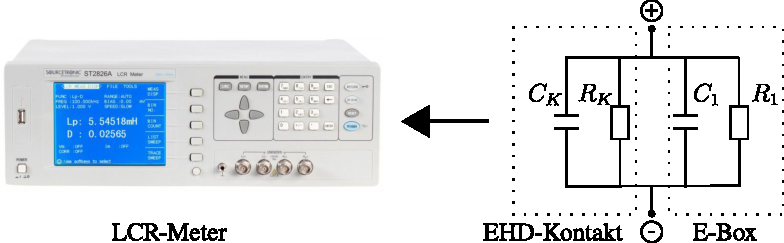
\includegraphics[]{./images/versuchsaufbau_mit_lcr_meter.pdf}
    \caption{Versuchsaufbau zur Kapazitätsmessung mit LCR-Meter}
    \label{fig:versuchsaufbau_zur_kapazitaetsmessung_mit_lcr_meter}
\end{figure}

Das LCR-Messgerät bietet einen breiten Frequenzbereich von \SI{20}{\Hz} bis \SI{50}{\MHz}.
Dank der Kelvin-Messproben hat das Gerät eine sehr gute Genauigkeit von \SI{0.1}{\percent} und ermöglicht die Messung auch bei kleinsten Änderung des Systems.
Mit einer Sinuskorrelationstechnik bietet das Gerät eine rauschfreie Analyse.
Abbildung \ref{fig:messprobe_eines_mit_dem_lcr_meter} zeigt das Messergebnis beim Referenz-Kondensator (\SI{3.3}{\nano\F}) mit dem LCR-Messgerät bei verschiedenen Frequenzen.
% ----------------------------------------
% Fig: Messprobe mit 3.3 nF mit dem LCR-Meter
% ----------------------------------------
\begin{figure}[htb]
    \centering
    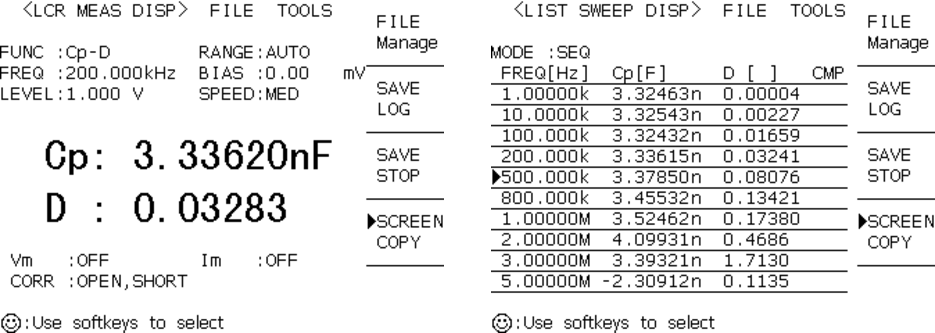
\includegraphics[]{./images/messprobe_mit_lcr_meter.pdf}
    \caption{Messergebnis eines Referenz-Kondensators mit dem LCR-Messgerät}
    \label{fig:messprobe_eines_mit_dem_lcr_meter}
\end{figure}

% ----------------------------------------
% Sec: Versuchdurchführung
% ----------------------------------------
\section{Versuchdurchführung}
\label{sec:versuchdurchfuehrung}
